\subsection{Introducción}
El cuarto sprint tiene como objetivo alcanzar el estado final de Resnet,
es decir, lograr que Centinela esté completamente funcional y lista para ser
utilizada por los usuarios. En el contexto del motor de búsqueda,
se espera que  Centinela sea capaz de realizar las búsquedas
que Resnet podía realizar en su estado final, alcanzando así el nivel de funcionalidad de la versión anterior.
\subsection{Objetivos}
\begin{itemize}
    \item Implementar la automatización para generar el Corpus y el Modelo de TF-IDF
    \item Implementar la funcionalidad de búsqueda de autores relevantes dado un tópico
    \item Implementar la funcionalidad de búsqueda de artículos relevantes dado un tópico
    \item Implementar la funcionalidad para obtener la red de coautoría de un autor
    \item Implementar la funcionalidad para obtener un Articulo dado su ID de Scopus
    \item Implementar la funcionalidad para obtener un Autor dado su ID de Scopus
\end{itemize}
\subsection{Planificación}
Para este sprint se terminaron las tareas que quedaron pendientes en el Sprint 1 (Ver sección \ref{chapter02-section02-sprint1})  y en el Sprint 2 (Ver sección \ref{chapter02-section02-sprint2}).
En la tabla \ref{C2T4:Historias de Usuario del Sprint 4} se presentan las historias de usuario que se abordarán en este sprint con sus respectivas tareas.
\begin{table}[!t]
    \centering
    \begin{tabular}{|p{2.5cm}|p{5cm}|p{6cm}|}
        \midrule
        \textbf{Identificador} & \textbf{Historia de Usuario}                                                                                                                                                                               & \textbf{Tareas} \\
        \hline
        HU-SE-01 & Como usuario no registrado deseo poder encontrar artículos relevantes dado un  tema de investigación para poder acceder rápidamente a información útil y actualizada que apoye mi estudio o trabajo        &
        \begin{compactitem}
            \item Generar el corpus \footnote{
                Conjunto de documentos que se utilizan para entrenar un modelo de \textit{Machine Learning} o \textit{Deep Learning}
            } de datos  
            \item Generar el modelo de TF-IDF a partir del corpus
            \item Crear el modelo de Artículo para la base de datos
            \item Implementar el filtro de artículos por año
            \item Crear un servicio de búsqueda de artículos
            \item Desarrollar un endpoint para manejar las solicitudes entrantes
        \end{compactitem}
        \\
        \hline
        HU-SE-04 & Como usuario no registrado quiero poder ver los artículos de un investigador para conocer su trabajo y las publicaciones en las que ha contribuido &
        \begin{compactitem}
            \item Implementar un endpoint para recuperar el perfil de un investigador y sus publicaciones
            \item Crear un servicio de búsqueda de investigadores y sus artículos
        \end{compactitem}
        \\
        \hline
        HU-SE-03 & Como usuario no registrado, deseo poder ver la red de coautoría de un autor para visualizar un grafo con los autores con los que ha colaborado, así como la fuerza de esas colaboraciones &
        \begin{compactitem}
            \item Implementar un endpoint para recuperar los datos de colaboración entre autores
            \item Crear un servicio que genere los datos del grafo de coautoría de un autor
        \end{compactitem}
        \\
        \hline
    \end{tabular}
    \caption{Historias de Usuario del sprint 4}
    \label{C2T4:Historias de Usuario del Sprint 4}
\end{table}


Los criterios de aceptación para las historias de usuario HU-SE-01, HU-SE-03 y HU-SE-04 han sido definidos y se pueden consultar en las siguientes figuras: Figura \ref{fig:aceptance-criteria-HU-SE-01}, Figura \ref{C2F2:Criterios de Aceptacion HU-SE-03} y Figura \ref{C2F2:Criterios de Aceptacion HU-SE-04}.
\subsection{Implementación}

Para la implementación de ciertas tareas en este Sprint, se optó por reutilizar el código de la versión anterior de ResNet, ya que se consideró más eficiente y rápido que comenzar desde cero.
La optimización de funcionalidades existentes no está incluida en el alcance de este componente.
Las funcionalidades que se reutilizarán son la generación del corpus y el modelo de TF-IDF,
dado que estas tareas son las más demandantes en términos de tiempo y se determinó que no era necesario reimplementarlas.
A estas funcionalidades solo se les añadirá una capa de infraestructura,
ya que la lógica de negocio ya está implementada en la versión anterior de ResNet.
Esto garantizará un punto de entrada para generar tanto el corpus como el modelo de TF-IDF,
permitiendo su utilización en las búsquedas de autores y artículos.

%% HU-SE-01
Tarea: \textit{HU-SE-01: Generar el corpus de datos}
Dado que las funcionalidades de buscar autores y artículos relevantes dependen del corpus de datos, y del modelo de TF-IDF, estas tareas se realizarán en primer lugar.
Para poder generar el corpus de datos, el endppoint \textit{/api/v1/generate-corpus/} se encargará de recibir la petición mediante el método POST.
Este llamara al caso de uso \textit{GenerateCorpusUseCase} que se encargará de generar de ejecutar la lógica de negocio para generar el corpus de datos.
El mismo que toma datos de Autores, Artículos, y Tópicos de la base de datos Neo4j para crear los documentos y almacenarlos en un archivo Pickle.
En la figura \ref{fig:sequence-diagram-generate-corpus} se muestra el diagrama de secuencia para la generación del corpus de datos.

\begin{figure}[H]
    \centering
    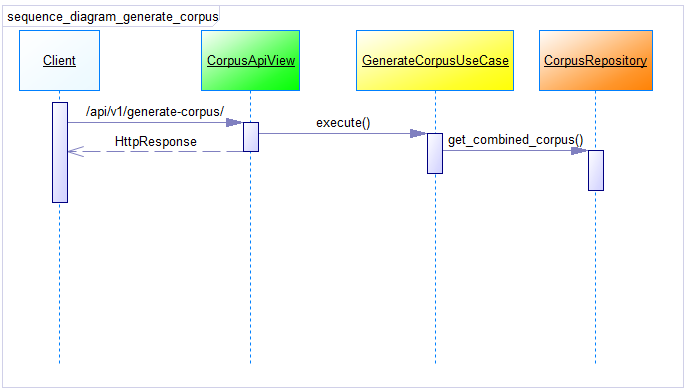
\includegraphics[scale=0.8]{../02Figures/02Chapter/Sprints/Sprint-4/sequence_diagram_generate_corpus.png}
    \caption{Diagrama de secuencia para la generación del Corpus}
    \label{fig:sequence-diagram-generate-corpus}
\end{figure}

Tarea: \textit{HU-SE-01: Generar el modelo de TF-IDF}
Una vez que el corpus de datos ha sido generado, se procederá a generar el modelo de TF-IDF.
Para ello, el endpoint \textit{/api/v1/generate-model/} se encargará de recibir la petición mediante el método POST.
Este llamara al caso de uso \textit{GenerateTfidfUseCase} que se encargará de ejecutar la lógica de negocio para generar el modelo de TF-IDF.
El mismo que toma el corpus de datos generado anteriormente y lo procesa para generar el modelo de TF-IDF, para guardar el modelo en un archivo Pickle.
En la figura \ref{fig:sequence-diagram-generate-tfidf} se muestra el diagrama de secuencia para la generación del modelo de TF-IDF.

\begin{figure}[H]
    \centering
    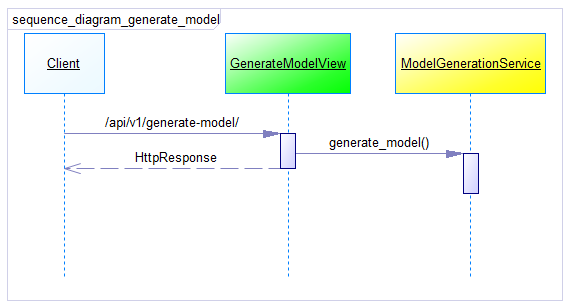
\includegraphics[scale=0.7]{../02Figures/02Chapter/Sprints/Sprint-4/sequence_diagram_generate_model.png}
    \caption{Diagrama de secuencia para la generación del Modelo de TF-IDF}
    \label{fig:sequence-diagram-generate-tfidf}
\end{figure}

Una vez que el corpus de datos y el modelo han sido generados se puede proceder a realizar las implementaciones tanto de autores relevantes como de artículos relevantes.
Para la funcionalidad de Artículos relevantes la ruta \textit{/api/v1/articles/most-relevant-articles-by-topic/} (POST) recibira en su cuerpo los siguientes datos:
\begin{itemize}
    \item query: El Tópico por el cual se desea buscar los Artículos relevantes
    \item size: El limite de Artículos que se desea obtener, por defecto es 10
    \item page: La pagina de Artículos que se desea obtener, por defecto es 1
    \item type: Si se desea incluir o excluir años de publicación
    \item years: Años de publicación a incluir o excluir
\end{itemize}
Este endpoint llamara al caso de uso \textit{GetMostRelevantArticlesByTopicUseCase} que se encargará de ejecutar la lógica de negocio para obtener los Artículos relevantes.
El proceso comienza tomando el tópico y pasándolo al modelo TF-IDF para identificar los IDs de los artículos relevantes. A continuación, se consulta la base de datos Neo4j para obtener los datos de esos artículos. Utilizando los parámetros de la petición, se buscan y retornan los artículos relevantes en una lista paginada, todo esto dentro de una respuesta Http.
En la figura \ref{fig:sequence-diagram-get-most-relevant-articles} se muestra el diagrama de secuencia para la obtención de los Artículos relevantes.

\begin{figure}[H]
    \centering
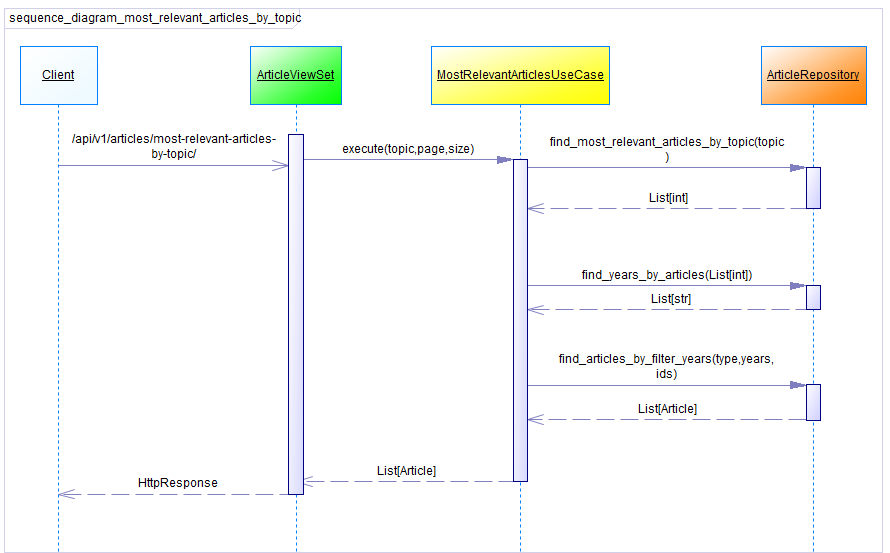
\includegraphics[scale=0.7]{../02Figures/02Chapter/Sprints/Sprint-4/sequence_diagram_most_relevant_articles_by_topic.png}
    \caption{Diagrama de secuencia para la obtención de los Artículos Relevantes}
    \label{fig:sequence-diagram-get-most-relevant-articles}
\end{figure}

%% HU-SE-03

HU-SE-03: Obtener la red de coautoría de un autor
Para la funcionalidad de obtener la red de coautoría de un autor, la ruta \textit{/api/v1/coauthors/coauthors/{id}/coauthors\_by\_id/} (GET) recibirá en su URL el ID del autor del cual se desea obtener la red de coautoría.
Este endpoint llamara al caso de uso \textit{GetCoauthorsByAuthorIdUseCase} que se encargará de ejecutar la lógica de negocio para obtener la red de coautoría de un autor.
El proceso comienza tomando el ID del autor y consultando la base de datos Neo4j para obtener los nodos (Autores) y links (collab\_strength) de la red de coautoría de ese autor. A continuación, se consultan los datos de esos coautores y se retornan en una respuesta Http.
En la figura \ref{fig:sequence-diagram-get-coauthors-by-author-id} se muestra el diagrama de secuencia para la obtención de la red de coautoría de un autor.
\begin{figure}[H]
    \centering
    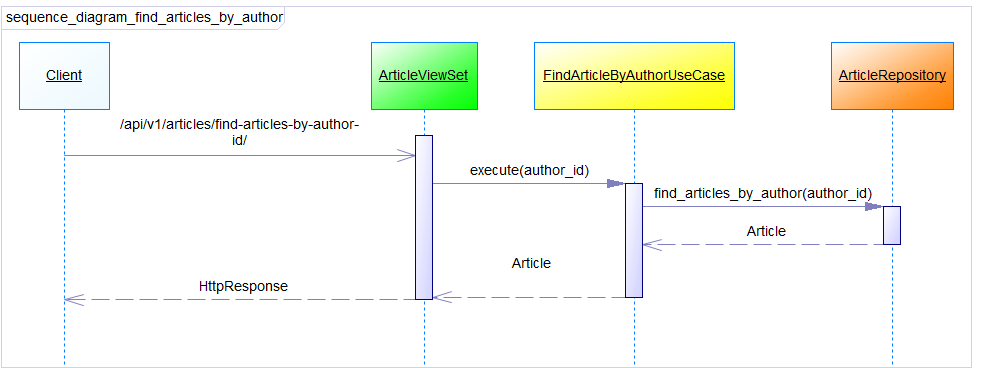
\includegraphics[scale=0.7]{../02Figures/02Chapter/Sprints/Sprint-4/sequence_diagram_find_articles_by_author.png}
    \caption{Diagrama de secuencia para la obtención de la red de coautoría de un autor}
    \label{fig:sequence-diagram-get-coauthors-by-author-id}
\end{figure}

%% HY-SE-04
HU-SE-03: Para obtener los Artículos en los que ha colaborado un autor, la ruta \textit{/api/v1/articles/find-articles-by-author-id/} (GET) recibirá en su URL el ID del autor del cual se desea obtener los articulos en los que ha colaborado.
Este endpoint llamara al caso de uso \textit{FindArticlesByAuthorIdUseCase} que se encargará de ejecutar la lógica de negocio para obtener los Artículos en los que ha colaborado un autor.
En la Figura \ref{fig:sequence-diagram-find-articles-by-author-id} se muestra el diagrama de secuencia para la obtención de los artículos en los que ha colaborado un autor.
\begin{figure}[H]
    \centering
    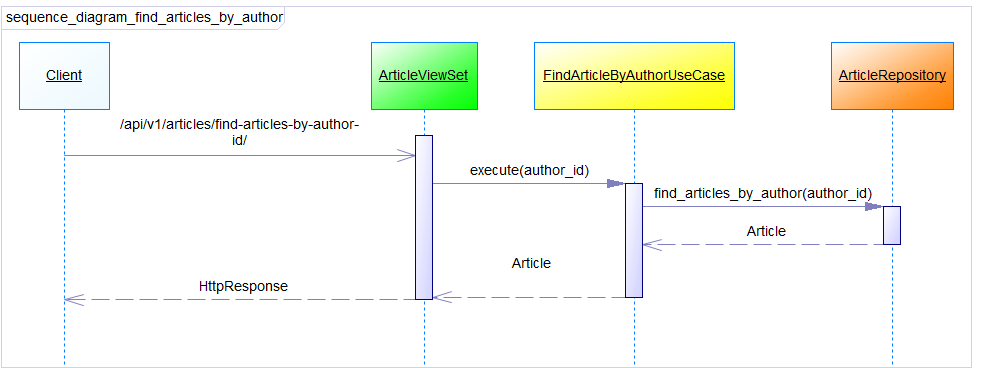
\includegraphics[scale=0.7]{../02Figures/02Chapter/Sprints/Sprint-4/sequence_diagram_find_articles_by_author.png}
    \caption{Diagrama de secuencia para la obtención de los Artículos en los que ha colaborado un autor}
    \label{fig:sequence-diagram-find-articles-by-author-id}
\end{figure}

\subsection{Revisión y Retrospectiva}
Al finalizar el sprint, se logró implementar las funcionalidades de búsqueda de autores y artículos relevantes, así como la obtención de la red de coautoría de un autor y la obtención de los artículos en los que ha colaborado un autor.
Mismas que habían quedado pendientes en los sprints anteriores. 
Así mismo, se logro evidenciar que la reutilización de código de la versión anterior de ResNet fue una buena decisión, ya que permitió acelerar el desarrollo de las funcionalidades.
También el uso de Arquitectura Hexagonal permitió diagramar de manera clara y concisa la implementación de las funcionalidades.
